% ==============================================================================
% DOCUMENT HEADER
% ==============================================================================

\documentclass[11t, a4paper, twocolumn]{article} 
\usepackage[english]{babel}
\usepackage{microtype}
\usepackage{amsmath,amsfonts,amsthm}
\usepackage[svgnames]{xcolor}
\usepackage[hang, small, labelfont=bf, up, textfont=it]{caption}
\usepackage{booktabs}
\usepackage{lastpage}
\usepackage{graphicx}
\usepackage{enumitem}
\setlist{noitemsep}
\usepackage{sectsty}
\allsectionsfont{\usefont{OT1}{phv}{b}{n}}
\usepackage{lipsum}
\usepackage{geometry}
\geometry{
	top=1cm,
	bottom=1.5cm,
	left=2cm,
	right=2cm,
	includehead,
	includefoot
}
\setlength{\columnsep}{7mm}
\usepackage[T1]{fontenc}
\usepackage[utf8]{inputenc}
\usepackage{XCharter}
\usepackage{fancyhdr}
\pagestyle{fancy}
\renewcommand{\headrulewidth}{0.0pt}
\renewcommand{\footrulewidth}{0.25pt}
\renewcommand{\sectionmark}[1]{\markboth{#1}{}}
\lhead{}
\chead{\textit{\thetitle}}
\rhead{}
\lfoot{}
\cfoot{}
\rfoot{\footnotesize Page \thepage\ of \pageref{LastPage}}
\fancypagestyle{firstpage}{
	\fancyhf{}
	\renewcommand{\footrulewidth}{0pt}
}
\newcommand{\authorstyle}[1]{{\large\usefont{OT1}{phv}{b}{n}\color{Black}#1}}
\newcommand{\institution}[1]{{\footnotesize\usefont{OT1}{phv}{}{sl}\color{Black}#1}}
\usepackage{titling}
\newcommand{\HorRule}{\color{Black}\rule{\linewidth}{0.75pt}}
\pretitle{
	\vspace{-30pt}
	\HorRule\vspace{10pt}
	\fontsize{30}{34}\usefont{OT1}{phv}{b}{n}\selectfont
	\raggedright
	\color{Black}
}
\posttitle{\par\vskip 15pt}
\preauthor{}
\postauthor{
	\vspace{10pt}
	\par\HorRule
	\vspace{5pt}
}
\usepackage{lettrine}
\usepackage{fix-cm}
\newcommand{\initial}[1]{
	\lettrine[lines=3,findent=4pt,nindent=0pt]{
		\color{DarkGoldenrod}
		{#1}
	}{}
}
\usepackage{xstring}
\newcommand{\lettrineabstract}[1]{
	\StrLeft{#1}{1}[\firstletter]
	\initial{\firstletter}\textbf{\StrGobbleLeft{#1}{1}}
}
\usepackage[backend=bibtex,style=numeric,natbib=true]{biblatex}
\addbibresource{ref.bib}
\usepackage[autostyle=true]{csquotes}


\title{Estimating real-time high street footfall from Wi-Fi probe requests}
\author{
	\authorstyle{
		Balamurugan Soundararaj\textsuperscript{1}, 
		James Cheshire\textsuperscript{1} and 
		Paul Longley\textsuperscript{1}}
	\newline\newline
	\textsuperscript{1}\institution{
		Department of Geography, 
		University College London, 
		United Kingdom}
}
\date{\today}

% ==============================================================================
% DOCUMENT BODY
% ==============================================================================

\begin{document}

	\maketitle
	\thispagestyle{firstpage}

	In the past decade Wi-Fi has emerged as the most
	commonly used technology in providing 
	internet access to mobile devices such as smartphones, tablets
	and laptops in public and private spaces.
	This has resulted in multiple Wi-Fi networks being available at
	almost every location in an urban environment.
	Traversing through this overlapping mesh of Wi-Fi networks,
	modern mobile devices with Wi-Fi antennae regularly
	broadcast special type of signals known as probe requests to
	discover available Wi-Fi networks and switch seamlessly
	between them.
	This is a hardware level signal which was standardised by IEEE 802.11b/g
	specification relays information about the source mobile device to
	any Access Points (AP) available around it.
	Since this is the first step in establishing
	a connection between any two devices, it is
	is universal to any device which uses a Wi-Fi radio to communicate.
	This makes these probe requests
	an open, passive, continuous, and wireless source of
	data available at any urban location which can provide us with clues in
	understanding the number of people present in the immediate surroundings
	in real-time with high granularity \citep{freud2015,konto2017}.
	In this paper, from a set of probe requests collected
	at a high street location in London,
	along with manually counted data, we demonstrate
	that pedestrian footfall can be estimated with considerable accuracy without
	infringing on the privacy of the mobile users involved.

	\begin{figure*}
		\begin{center}
			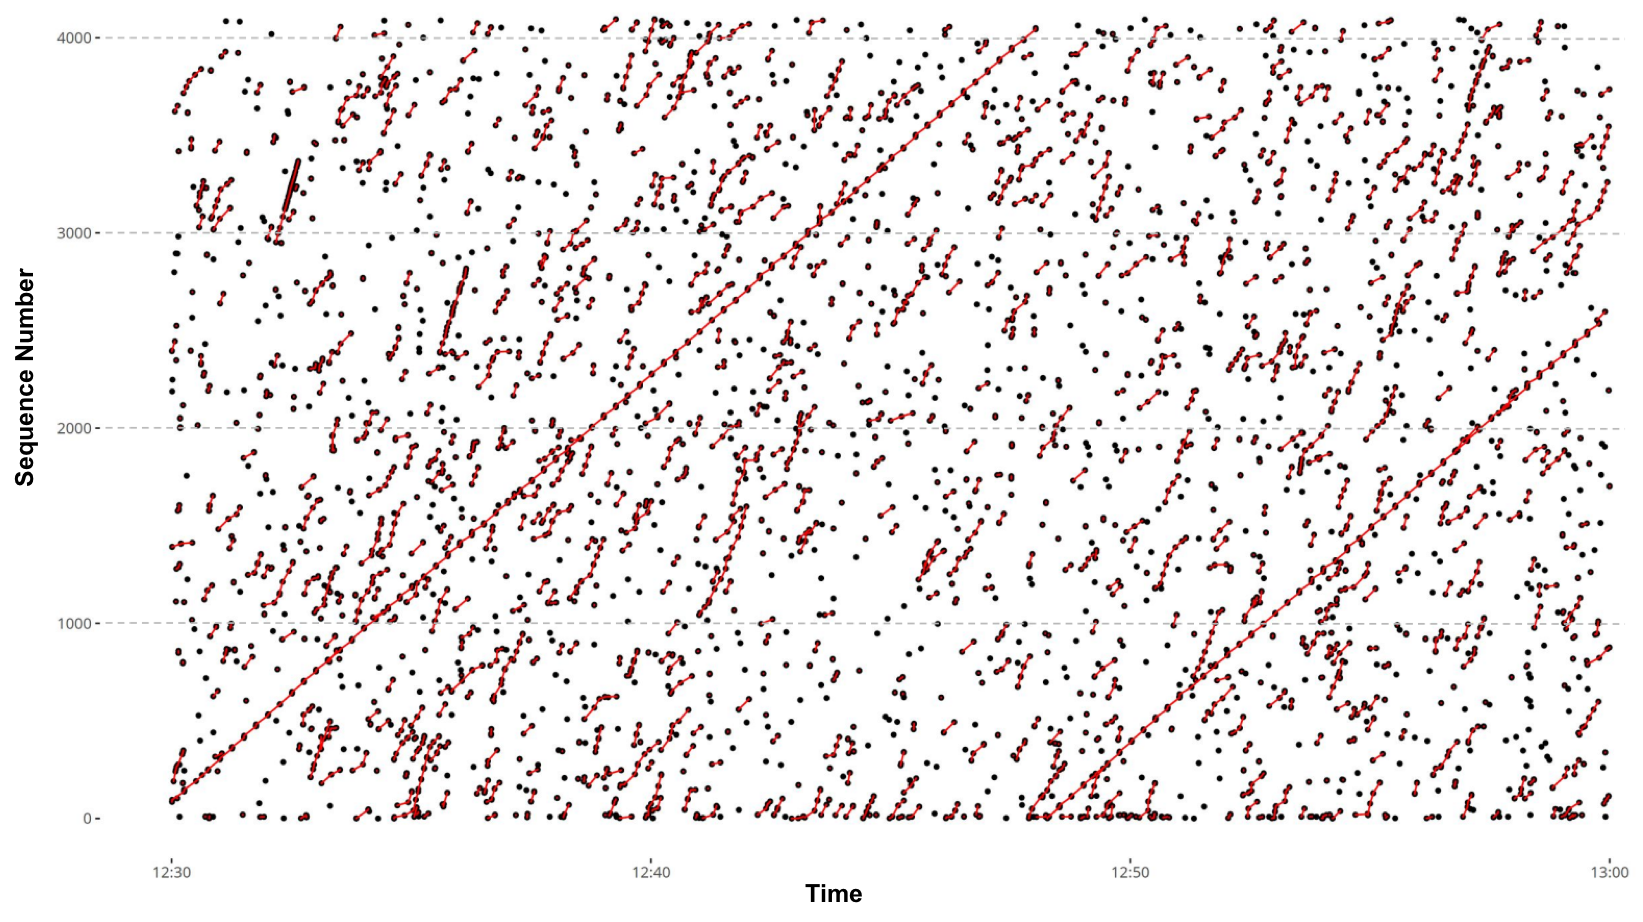
\includegraphics
				[width=0.8\textwidth,trim=4 4 4 4,clip]
				{outputs/clustering_2.png}
			\caption{Clustering probe requests based on increasing sequence
			numbers present in them.}
			\label{fig}
		\end{center}
	\end{figure*}

	There have been numerous attempts at using Wi-Fi
	to measure the volume and movement of people in built environment for various
	applications \citep{zarim2006,sap2015,reki2007}.
	Though most research observe feasible and favorable results,
	in recent years, one of the major challenges faced in such attempts
	has been the MAC address randomisation process.
	This process aims to protect the users' privacy by anonymising
	the only globally identifiable portion of the probe requests
	resulting in a set of probe requests generated by the same device
	with different random MAC addresses \citep{green2008}.
	There have been various successful research in breaking this
	randomisation process to extract real MAC addresses \citep{martin2017}
	but this usually results in serious risk in infringement of
	privacy of the users of the mobile devices.
	There is a clear gap in the research for exploring methodologies
	which enables us to estimate the number of unique mobile
	devices from a set of anonymised probe requests
	without the need to reveal their original MAC addresses.

	A pilot survey was conducted at Oxford street in London
	on 20 December 2017 from 12:30 to 13:00 where two sets of data
	were collected on pedestrian footfall through Wi-Fi sensing
	and manual counting in parallel.
	The Wi-Fi sensor collected all the probe requests that were 
	broadcast around the area and recorded
	the time-stamp at which they were collected,
	MAC address of the source mobile device
	(anonymised using a hashing algorithm),
	organisationally unique identifier (OUI) of the manufacturer of the device,
	total length of the signal in bits,
	the strength of the signal reported by the mobile device in dBm,
	the sequence number of the signal,
	duration for which the signal was transmitted, 
	the service set identifier (SSID) of the access point targeted
	by the probe request and 
	the length of the extra information (tags) embedded in the packets.
	The manual count was done by an android application on a mobile phone
	which records the time-stamp every time the surveyor touches the screen
	which corresponds to one pedestrian footfall on the sidewalk.

	Being one of the busiest location in the United Kingdom, the location
	generated approximately 60,000 probe requests in the 30 minutes
	interval through the Wi-Fi sensor and 3,722 people were counted manually.
	When we aggregate the probe requests by their MAC address for every minute,
	the difference between the sensor counts and the manual counts
	is observed to be on average 425\%. 
	This shows that there is a large amount of noise
	in the data which might include signals from devices outside the area where
	the manual count was conducted and the anonymised probe requests from the
	same devices with different MAC addresses.
	Before we go look at the data
	in detail, an initial analysis shows that the fields - SSID and tags are
	very sparse and doesn't provide much information for our cleaning process 
	and the duration field is closely related to the length of the 
	probe request and provides no new information.
	So we remove these fields from further analysis.

	We remove the noise from devices outside the area of interest 
	by removing all the probe requests which report a "low" signal strength.
	This classification of "high" vs "low" is done through "k-means"
	classification algorithm.
	The cutoff point for the collected data is -71dBm.
	This process of filtering is highly effective and reduces the difference
	between the sensor counts and manual counts to 30\%. We observe that
	around 55\% of all probe requests collected are anonymised.
	We assign the hashed MAC address the unique identifier for the rest of
	the 45\% and investigate the anonymised probe requests further.
	
	We then use the fields - OUI, lengths and sequence number,
	to tackle the noise from devices which anonymising the probe requests.
	OUI and length are used to split the dataset into
	groups of probe requests from similar
	devices and each subset is classified further
	based on a graph based clustering algorithm 
	where each cluster corresponds to an unique device.
	The algorithm works by creating a graph where the probe requests
	are the nodes and the links are created
	between them based on the following rules,

	\begin{enumerate}
		\item A link can go only forward in time.
		\item A link can exist between nodes with a 
			maximum time difference of $\alpha$ (time threshold)
		\item A link can go from low to high sequence numbers.
		\item A link can exist between nodes with a
			maximum sequence number difference of $\beta$ (sequence threshold)
		\item A node can have only one incoming link and outgoing link
			which is the shortest of all possible such links.
	\end{enumerate}

	The nodes are then classified based on the unique connected component they
	belong to. This classification is assigned as the unique identifier for the
	anonymised probe requests.
	Figure \ref{fig} shows the clustering process for where the black dots show
	probe requests and red lines connecting them show the clusters
	corresponding to the same device generated them.
	We finally combine both normal and anonymised probe requests, 
	aggregate them based on their unique identifier and remove
	repeating probe requests which reduces the difference between
	the sensor counts and the manual counts to -18\%.

	It is important to note that the filtering process is done based on just
	the information present in the probe requests
	and their temporal distribution.
	This makes sure that though the mobile devices are uniquely identified
	there is no more personal data is generated linking the probe requests
	to the users of the mobile devices. This method essentially gives us a
	way to estimate the footfall in real-time without identifying or tracking the
	mobile devices themselves.

	This Wi-Fi based footfall counting methodology offers a large number of
	applications and benefits. Since Wi-Fi based sensors are inexpensive and the
	data model is scalable, it is readily possible to use this methodology for
	a large network of sensors to gather granular data on pedestrian footfall.
	Projects such as Smart Street Sensors, can utilise the methodology to
	overcome the challenges introduced by implementation of MAC address
	randomisation. Such precise and granular data also enables us in confidently
	model the pedestrian flow in urban road networks and will be indispensable
	tool in the smart city framework. This can also be used in understanding and
	classifying geographical areas based on the spatio temporal distribution of
	the volume of activity in them.

	\printbibliography[title={References}]

\end{document}
